\documentclass{article}
\usepackage[left=2cm,right=2cm,top=1.5cm,bottom=1.5cm]{geometry} 
\usepackage{enumitem}
\usepackage[francais]{babel}
% \usepackage{caption}
\usepackage{hyperref}
\hypersetup{
    colorlinks = true,
    urlcolor = {blue}
}
\usepackage{graphicx}
\usepackage[dvipsnames]{xcolor}
\usepackage[utf8]{inputenc}
\usepackage[T1]{fontenc} %Permets l'utilisation des guillemets « et »
\begin{document}
\begin{center}
\LARGE{\bf \underline {Terminal Ubuntu :}} \\
\end{center}
First of all, the Ubuntu terminal is a terminal that run appart of windows.
\\ So if you want to navigate trough your documents, you need to go to de root and begin by /mnt. \\
\\ There's a few basics commands that can be useful : \\
\begin{itemize}
    \item \textcolor{red}{cd} (change directory) \\
    \item \textcolor{red}{echo} (allows you to write content in a file > to erase content and add new, >> to do a new line) \\
    \item \textcolor{red}{ls} (List of the elements inside a folder) [Equivalent on windows DIR] \\
    \item \textcolor{red}{pwd} (Show the path of the forlder we are) [CD on windows] Print working directory \\
    \item \textcolor{red}{cd ..} (To get back in the path) \\
    \item \textcolor{red}{mkdir} (create a folder at the place) \\
    \item \textcolor{red}{touch} (check if a file with the name exist, if not create one) \\
    \item \textcolor{red}{cat} (cat command allows you to create single or multiple files, view content of a file, concatenate files and redirect output in terminal or files.) \\
    More explication with the command cat, if you use the command cat to create a file, cat > name.file you can write multiple lines in it directly after. \\
    However you need to quit after with ctrl + d (or with ctrl + c but it's not recommanded). \\
    \item \textcolor{red}{mv} (allows you to move a file into a folder you can also use this command to rename a folder if you don't move it the second entrance is the new name) [exemple : mv one.txt story] \\
    \item \textcolor{red}{rm} (allow you to delete a file, you need to confirm that) \\
    \item \textcolor{red}{rm -rf} (delete the directory and all inside) \\
    \item \textcolor{red}{cp} (allows you to copy a file) [exemple : cp one.txt two.txt] \\
    \item \textcolor{red}{dirs / pushd / popd} (pushd allows you to add a path to a stack that will be keep in memory. dirs allows you to see the stack and popd to remove the last path added.) \\
    If we want to add a path to the stack without going to this path, we can type \textcolor{red}{pushd -n « fullpath »} \\
    You can use the options \textcolor{red}{-l} and \textcolor{red}{-v} with dirs to make the appears as an enumerate list. \\
    So you can more easely use the pushd command with indices to go on the path you want. \\
    You can also use popd with an indice to choose the path you want to delete from the stack. \\
    \item \textcolor{red}{ls -s} (allows you to see the owner and group permissions of the files) \\
    To change owner of a file you need the admin privilege. \\
    \item \textcolor{red}{sudo} (Allows you to run command as root) \\
\end{itemize}
\begin{minipage}[c]{0.5\textwidth}
    \begin{itemize}
        \item \textcolor{red}{chown} (Allows you to change the owner of a file) \\
        \item \textcolor{red}{chmod} (control who can access file) \\
        \item \textcolor{red}{chgrp} (Allows you to change the group of the file)
    \end{itemize}
\end{minipage}
\begin{minipage}[c]{0.05\textwidth}
    \Bigg \}
\end{minipage}
\begin{minipage}[c]{0.45\textwidth}
    you cannot use \textcolor{red}{chonw, chmod, chgrp} on windows files when you're in a linux terminal
\end{minipage} \\ \\
\begin{itemize}
    \item For the command \textcolor{red}{chmod} you can use these options : \\
    \begin{center}          
        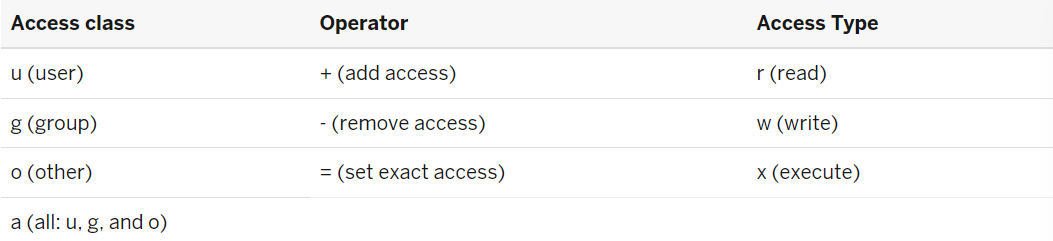
\includegraphics[scale=0.7]{chmod.png} \\ \vspace{0.3cm}
        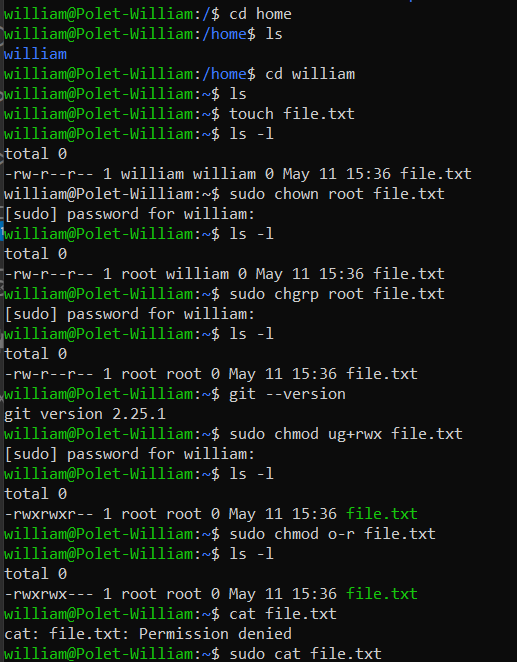
\includegraphics[scale=1]{chmodTerminal.png}
    \end{center}
    It's normal if there's one line missing that's because the file was empty so the cat command return nothing.
\end{itemize}

%-------------------------------- NEW PAGE --------------------------------
\newpage
\begin{center}
    \LARGE{\bf \underline {Nano and Vim :}} \\
\end{center}
Nano and Vim are text editors that can be used inside the terminal. \\ \\
To create a file with Nano, type \textcolor{red}{nano « name.extension »} and then a windows appears. \\
\begin{center}
    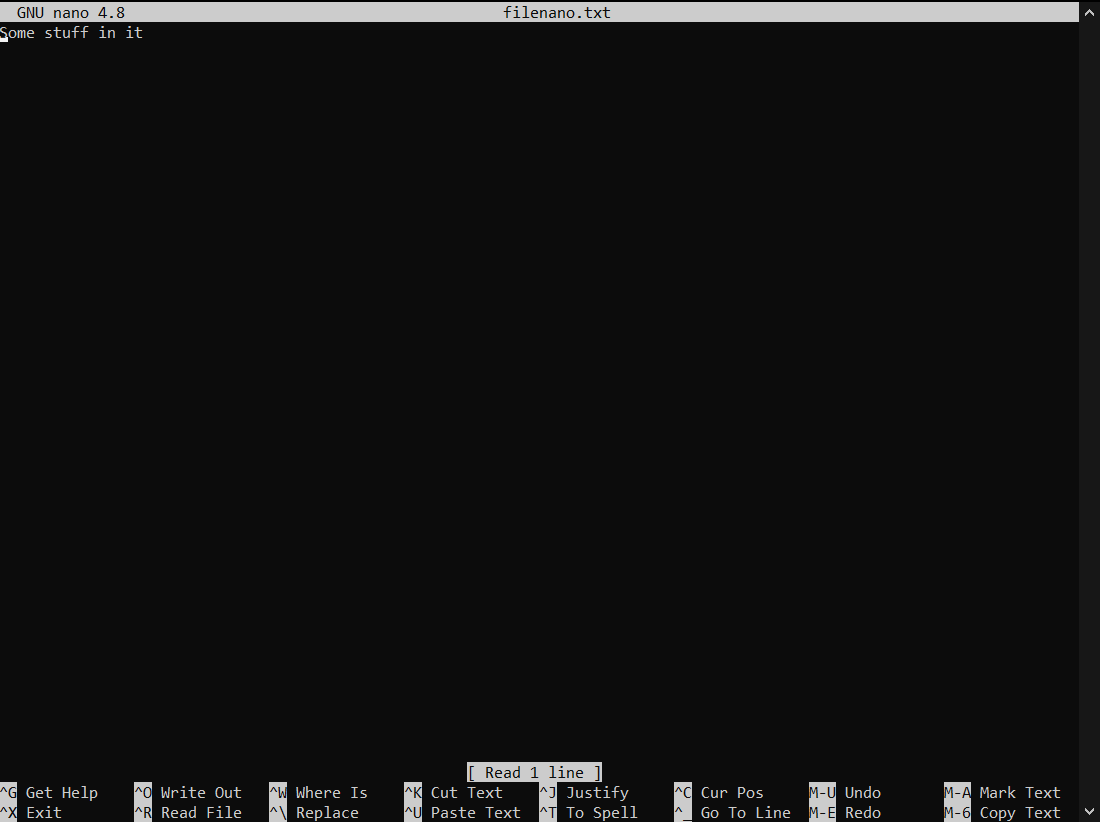
\includegraphics[scale=0.45]{Nano.png}
\end{center}
You can write in it, to save it you need to use \textcolor{ForestGreen}{ctrl + O} and press enter to confirm, after you quit with \textcolor{ForestGreen}{ctrl + X} \\ \\
To create a file with Vim use the same way, type \textcolor{red}{vim « name.extension »} \\
You will have a window that appears and to \textcolor{ForestGreen}{write} in it you need to press \textcolor{ForestGreen}{i} to enter in insert mode. When you have finish you can press \textcolor{ForestGreen}{esc} to stop editing. \\
To save the file type \textcolor{red}{:wq} (to save and exit the file) to only exit the file type \textcolor{red}{:q!} \\
There's a lot of things to learn from Vim, for a little preview you can type the command \textcolor{red}{vimtutor}. \\
For exemple you can use the command \textcolor{red}{dw} in normal mode to delete an entire word, or juste use the \textcolor{ForestGreen}{x} to delete a caracter. \\ \\
\begin{center}
    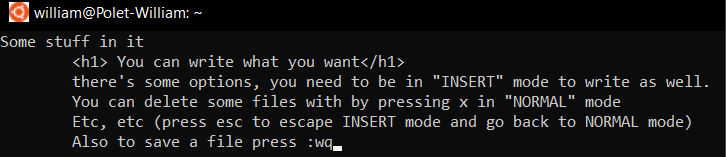
\includegraphics[scale=1]{Vim.png}
\end{center}
\begin{minipage}[c]{0.55\textwidth}
    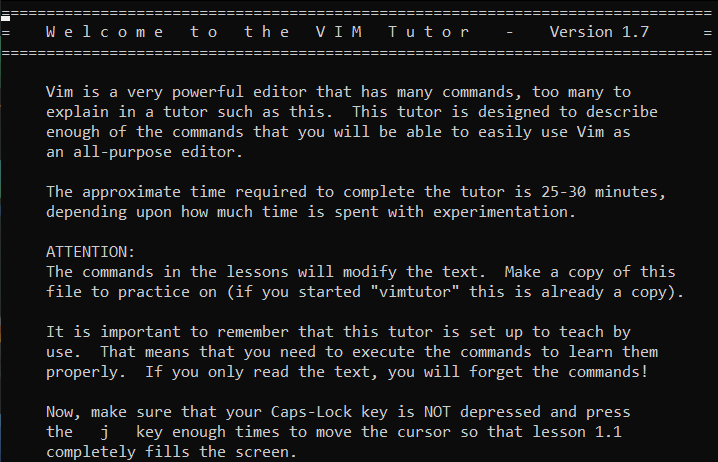
\includegraphics[scale=0.6]{VimTutor1.png}
\end{minipage}
\begin{minipage}[c]{0.5\textwidth}
    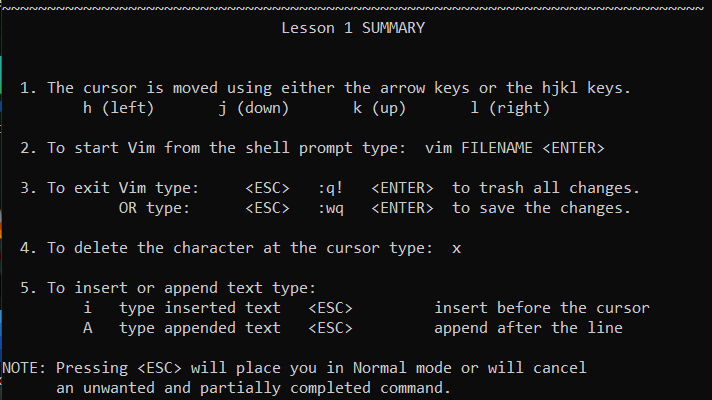
\includegraphics[scale=0.6]{VimTutor2.png}
\end{minipage}

%-------------------------------- NEW PAGE --------------------------------
\newpage
\begin{center}
    \LARGE{\bf \underline {Markdown Langage :}} \\
\end{center}
Markdown is a lightweight langage for creating formatted text. \\
You can do it with any text editor. You just need to respect the syntax and use the extension .md \\
Few exemple of the syntax :
\begin{itemize}
    \item \textcolor{blue}{\#} is to make a title. You can put up 1 to 6 \textcolor{blue}{\#} (1 for the largest title and 6 for the smallest)
    \item To create a paragraph just write, if you want to go to the line, finish your line with 2 spaces.
    \item To make a list, just do a list who begin with \textcolor{blue}{1.} continue with \textcolor{blue}{2.} and if you want to do a sublist repeat usting \textcolor{blue}{1.} with an indentation.
    \item If you want to instert a gif use \textcolor{blue}{![  ]()} and the link of the gif between the parenthesis.
\end{itemize}
\begin{center}
    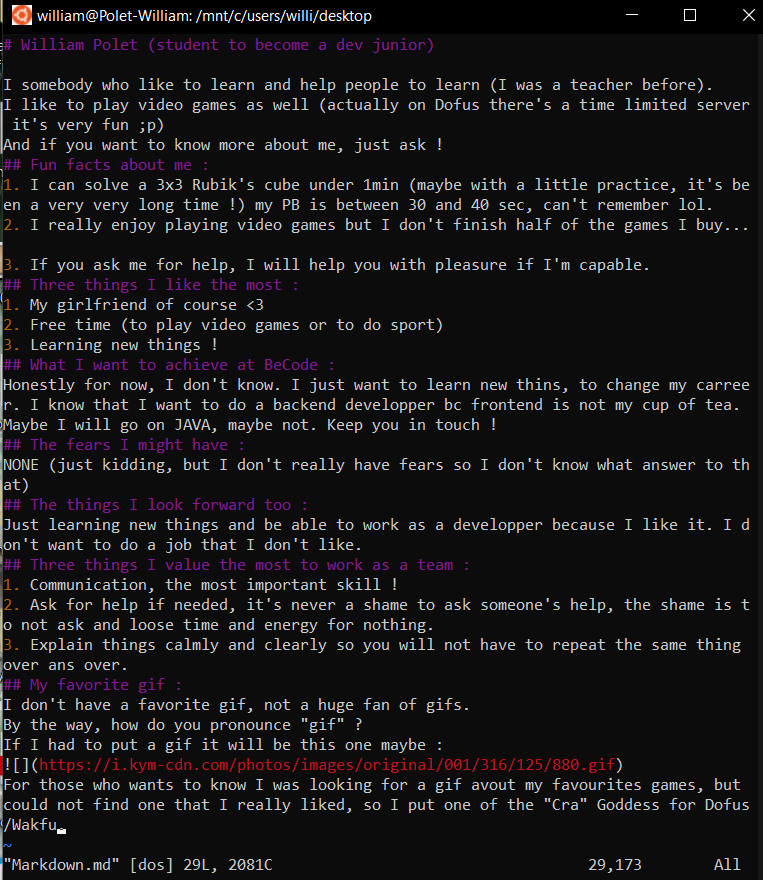
\includegraphics[scale=1]{VimMarkdown.png}    
\end{center}
And you can see the result by clicking on \href{https://github.com/WillPolet/Markdown}{this link}.
%-------------------------------- NEW PAGE --------------------------------
\newpage
\begin{center}
    \LARGE{\bf \underline {Git and Github :}} \\
\end{center}
Github is a service to store your code, git it's the technology that has two purpose. First one is to connect to the services (Github or BitBucket) \\
Second you will able to use git to do some version control, if you are writting a piece of code for 3 days for exemple. \\
You need to add something with no link, and we need to be sure that you don't have any issues, for that you can do a copy of your code and work on the copy. \\
Github online, git on your machine. \\
A repository is the place where you're going to push your code on Github. \\
It's nice to separate things, so one challenge, one repo. \\
\\ Create a new repository :
\begin{itemize}
    \item Choose repository name.
    \item Write a little description (optionnal)
    \item choose if it's public or private
    \item Add a README file, are the files that contains the description of the repo.
    \item Git ignore, just ignore certains files that you don't want to be on Github. (very important)
    \item Choose a license (MIT license is good), it's not a mandatory, it's a sentence that will protect your code (law ?)
\end{itemize}
(Github copilot is a help to code when we write, it's a paid service based on IA, that use the code on Github to perfect the IA and predict the code you will write.) \\ \\
So now whe have a repo with a README file, but it's only on github, we want to have it on our computer. \\
To do that, you need to create a link between your computer and the github repo. For that go on your repository and clone your repository, by HTTPS, SSH or Github CLI way. \\
CLI is a webservices software that you can install to your terminal to communicate for Github. It's a proprietary version of Git. \\ \\
Copy the HTTPS link, write \textcolor{red}{git clone « link from Github »} \\
Now we have a folder with the README file and in the file the title of the repo. \\
We can modify the README file, by adding some content. However it's only modify on the computer and not on Github. \\ \\
We need to keep the modification, so we want to put it on Github. \\
The folder (copy of your repo) is tracked by Git, actually on the main branch, the only one actually. \\
If you want to check if you modified the code you can type the command \textcolor{red}{git status} it gives you all the files modified. \\ \\
\textcolor{red}{git add .} the . is to say that I want to add everything. \\
(It put all the content in the bus and we can check if it has been added with git status) \\
\textcolor{red}{git commit -m} here -m is a flag (option to be more precise on the command) \\
When we do a git commit -m we need to put a message with it, we can for example say what we did in the repo or code. \\
(Now the little cross disappear but the bus is ready to go to Github) \\
\textcolor{red}{git push} It's the command to send the work on Github, but we need to tell where it needs to go. \\
For that we use \textcolor{red}{git remote -v} to have the address (that we copy earlier from Github) of the repo, but it's also caller « origin » \\
So we can do : \textcolor{red}{git push origin main} main is to say that the content need to go on the main branch. \\ \\
Let's do a little recap : 
\begin{itemize}
    \item do a clone of the repo. (\textcolor{red}{git clone}) (only if you have created a new repo)
    \item add content in the copy, new file, modify files who already exist, etc.
    \item add all the content to be send. (\textcolor{red}{git add .})
    \item give a message. (\textcolor{red}{git commit -m})
    \item send it to Github. (\textcolor{red}{git push origin main})
\end{itemize}
With git add, we can choose the files that we add. (But it not happen in general) \\
Difference between Master and Main, Master is just an old word for Main. \\
\newpage
\noindent\textbf{\underline{Initiate a repo with git init :}} \\ \\
To initialize a repo with git init, go to the folder in your terminal, write \textcolor{red}{git init}. \\
At every time remember that you can use the command \textcolor{red}{git status} to verify the status of your files. \\
To track your files, use as usual the command \textcolor{red}{git add .}, after that you can \textcolor{red}{git commit -m "your message"} \\ \\
\textcolor{blue}{First time it will ask you to login and run the commands \textcolor{red}{git config --global user.email "youremail@email.com"} \\
and the command \textcolor{red}{git config --global user.name "Your Name"}, personally for the name I put my Github UserName} \\ \\
Next you need to change the name of the branch : \textcolor{red}{git branch -M main} and add the link to the repository : \textcolor{red}{git remote add origin git@github.com:WillPolet/RepoName.git} \\ \\
After that you can \textcolor{red}{git push origin main}, but be aware, if there was a README file into your repo created on github, this will cause a problem, here's how to solve it : \\
Type these six commands in your terminal to install gh.
{
\color{blue}%
\begin{verbatim}
type -p curl >/dev/null || (sudo apt update && sudo apt install curl -y)

curl -fsSL https://cli.github.com/packages/githubcli-archive-keyring.gpg | sudo dd of=/usr/share
/keyrings/githubcli-archive-keyring.gpg \

&& sudo chmod go+r /usr/share/keyrings/githubcli-archive-keyring.gpg \ 

&& echo "deb \[arch=\$(dpkg --print-architecture) signed-by=/usr/share/keyrings/githubcli-archive
-keyring.gpg\] https://cli.github.com/packages stable main" | sudo tee /etc/apt/sources.list.d/
github-cli.list > /dev/null \ 

&& sudo apt update \ 

&& sudo apt install gh -y 
\end{verbatim}
}
After you need to authentificate with gh with \textcolor{red}{gh auth login}, choose to login through HTTPS or SSH (had an issue with HTTPS so I did it with SSH after). \\ \\
Very important, if you already had a README file, now you need to pull it by using this command : \textcolor{red}{git pull origin main --allow-unrelated-histories}. \\
And now you should be able to \textcolor{red}{git push origin main} \\ \\
So if there's no troubles, follow the instructions below, if there's a problem search in this document, if the problem persist go on google. \\ \\
\begin{itemize}
    \item Create a README.md file in your folder (optionnal)
    \item \textcolor{red}{git init}
    \item \textcolor{red}{git add .}
    \item \textcolor{red}{git commit -m}
    \item \textcolor{red}{git branch -M main}
    \item \textcolor{red}{git remote add origin git@github.com:WillPolet/RepoName.git}
    \item \textcolor{red}{git push -u main origin} -u is optionnal
\end{itemize}
\vspace{0.3cm}
If you don't have create your repo on Github yet, you can type this command after your commit : \\
\textcolor{red}{gh repo create my-newrepo --public --source=. --remote=upstream --push} \\
After that no need to do another command line, your files will be on your fresh new Github repo !
%-------------------------------- NEW PAGE --------------------------------
\newpage
\begin{center}
    \LARGE{\bf \underline {HTML sementic :}} \\
\end{center}
Sementic HTML is a way to build an HTML file with html tag that describes what it does. \\
Exemple of tags that you will use in these kind of document : \\ \\
\begin{minipage}[c]{0.25\textwidth}
    \begin{itemize}[label = $\bullet$]
        \item h1
        \item h2
        \item blockquote
        \item q
    \end{itemize}
\end{minipage}
\begin{minipage}[c]{0.25\textwidth}
    \begin{itemize}[label = $\bullet$]
        \item q
        \item img
        \item hr
        \item figure
    \end{itemize}
\end{minipage}
\begin{minipage}[c]{0.25\textwidth}
    \begin{itemize}[label = $\bullet$]
        \item caption
        \item table
        \item th
        \item tr
    \end{itemize}
\end{minipage}
\begin{minipage}[c]{0.25\textwidth}
    \begin{itemize}[label = $\bullet$]
        \item td
        \item ul
        \item ol
        \item li
    \end{itemize}
\end{minipage}
\vspace{0.3cm} \\
And there's way more !
\end{document}